\csname @openrightfalse\endcsname
\chapter{Curvature free differential geometry}
\chaptermark{Curvature free}

The reader should be familiar 
with the notions of smooth manifolds, 
Riemannian metrics and symplectic forms.

%%%%%%%%%%%%%%%%%%%%%%%%%%%%%%%%%%%%%%%%%
\subsection*{Distant involution}
\label{Distant involution}

\begin{pr}
Construct a Riemannian metric $g$ on $\mathbb{S}^3$ and an involution $\iota\:\mathbb{S}^3\z\to\mathbb{S}^3$ such that $\vol (\mathbb{S}^3,g)$ is arbitrary small and 
\[|x\z-\iota(x)|_g>1\]
 for any $x\in\mathbb{S}^3$.
\end{pr}

%%%%%%%%%%%%%%%%%%%%%%%%%%%%%%%%%%%%%%%%%%%%%%%%%%

\parit{Semisolution.}
Given $\eps>0$, construct a disk $\Delta$ in the plane with 
\[\length\partial \Delta<10\ \ \text{and}\ \ \area \Delta<\eps\]
that admits an continuous involution $\iota$ such that 
\[|\iota(x)-x|\ge 1\]
for any $x\in\partial \Delta$.

\begin{wrapfigure}{o}{20 mm}
\vskip-0mm
\centering
\includegraphics{mppics/pic-402}
\end{wrapfigure}

An example of $\Delta$ can be guessed from the picture;
the involution $\iota$ makes a length preserving half turn of its boundary $\partial \Delta$.


Take the product $\Delta\times \Delta\subset \RR^4$;
it is homeomorphic to the 4-ball.
Note that 
$$\vol_3[\partial(\Delta\times \Delta)]=2\cdot\area \Delta\cdot\length \partial \Delta<20\cdot\eps.$$
The boundary $\partial(\Delta\times \Delta)$ is homeomorphic to $\mathbb{S}^3$
and the restriction of the involution $(x,y)\z\mapsto (\iota(x),\iota(y))$ has the needed property.

All we have to do now is to smooth $\partial(\Delta\times \Delta)$ a little bit.
\qeds

This example is given by Christopher Croke \cite{croke}.
Note that according to Gromov's systolic inequality \cite{gromov-filling}, 
the involution $\iota$ above cannot be made isometric.

The following problem states that a similar construction is not possible for $\mathbb{S}^2$. 


%%%%%%%%%%%%%%%%%%%%%%%%%%%%%%%%%%%%%%%%%
\subsection*{Another distant involution}
\label{Another distant involution}

\begin{pr}
Given $x\in \mathbb{S}^2$, denote by $x'$ its antipodal point.
Suppose that $g$ is a Riemannian metric on $\mathbb{S}^2$ such that
\[|x-x'|_g\ge1\]
for any $x\in\mathbb{S}^2$.
Show that the area of $(\mathbb{S}^2,g)$ is bounded below by a fixed positive constant. 
\end{pr}

The expected solution uses Besicovitch inequality described in the next problem.

%???

%%%%%%%%%%%%%%%%%%%%%%%%%%%%%%%%%%%%%%%%%
\subsection*{Besicovitch inequality}
\label{Besicovitch inequality}

\begin{pr}
Let $g$ be a Riemannian metric on an $m$-dimensional cube $Q$ such that any curve connecting opposite faces has length at least $1$. 
Prove that 
\[\vol(Q,g)\ge 1,\] 
and the equality holds if and only if $(Q,g)$ is isometric to the unit cube.
\end{pr}



%%%%%%%%%%%%%%%%%%%%%%%%%%%%%%%%%%%%%%%%%
\subsection*{Minimal foliation\thm}
\label{gromomorphic-curves}

Minimal surfaces in Riemannian manifolds are defined on page \pageref{minimal surface}.

\begin{pr}
Consider the product of spheres $\mathbb{S}^2\times \mathbb{S}^2$ equipped with a Riemannian metric $g$ that is $C^\infty$-close to the product metric. 
Prove that there is a conformally equivalent metric $\lambda\cdot g$ and a re-parametrization of $\mathbb{S}^2\times \mathbb{S}^2$
such that for any $x,y\in \mathbb{S}^2$, the spheres $\{x\}\times\mathbb{S}^2$ and $\mathbb{S}^2\times \{y\}$ are minimal surfaces 
in $(\mathbb{S}^2\times \mathbb{S}^2,\lambda\cdot g)$.
\end{pr}


The expected solution requires pseudo-holomorphic curves introduced by Mikhael Gromov \cite{gromov-pseudoholomorphic}.

%%%%%%%%%%%%%%%%%%%%%%%%%%%%%%%%%%%%%%%%%
\subsection*{Volume and convexity\thm}
\label{Volume and convexity} 

A function $f$ defined on a Riemannian manifold is called convex if for any geodesic $\gamma$, the composition $f\circ\gamma$ is a convex real-to-real function.

\begin{pr}
Let $M$ be a complete Riemannian manifold that admits a non-constant convex function. 
Prove that $M$ has infinite volume.
\end{pr}

The expected solution uses Liouville's theorem about phase volume.
It implies in particular, that the geodesic flow on the unit tangent bundle of a Riemannian manifold preserves the volume.


%%%%%%%%%%%%%%%%%%%%%%%%%%%%%%%%%%%%%%%%%
\subsection*{Sasaki metric}
\label{pr:Sasaki metric}

Let $(M,g)$ be a Riemannian manifold.
The Sasaki metric is a natural choice of Riemannian metric $\hat g$ on the total space of the tangent bundle $\tau\:\T M\to M$.
It is uniquely defined by the following properties:
\begin{itemize}
\item The map $\tau\:(\T M,\hat g)\to (M,g)$ is a Riemannian submersion.
\item The metric on each tangent space $\T_p\subset \T M$ is the Euclidean metric induced by $g$.
\item Assume that $\gamma(t)$ is a curve in $M$ and $v(t)\in\T_{\gamma(t)}$ is a parallel vector field along $\gamma$. 
Note that $v(t)$ forms a curve in $\T M$.
For the Sasaki metric, we have $v'(t)\perp \T_{\gamma(t)}$ for any $t$;
that is, the curve $v(t)$ normally crosses the tangent spaces $\T_{\gamma(t)}\subset \T M$.
\end{itemize}

In other words, we identify the tangent space 
$\T_u[\T M]$ for any $u\z\in \T_p M$ with the direct sum of vertical and horizontal subspaces $\T_p M\z\oplus \T_p M$.
The projection of this splitting is defined by the differential $d\tau\:\T\T M\to \T M$
and we assume that the velocity of a curve in $\T M$ formed by a parallel field along a curve in $M$ is horizontal.
Then $\T_u[\T M]$ is equipped with the metric $\hat g$ defined by
\[\hat g(X,Y)=g(X^V,Y^V)+g(X^H,Y^H),\]
where $X^V$ and $X^H\in\T_pM$ denote the vertical and horizontal components of $X\in\T_u[\T M]$.



\begin{pr}
Let $g$ be a Riemannian metric on the sphere $\mathbb{S}^2$.
Consider the tangent bundle $\T \mathbb{S}^2$ 
equipped with the induced Sasaki metric $\hat g$.
Show that
the space $(\T \mathbb{S}^2, \hat g)$ lies at bounded distance to the ray $\RR_+=[0,\infty)$ in the sense of Gromov--Hausdorff.
\end{pr}


%%%%%%%%%%%%%%%%%%%%%%%%%%%%%%%%%%%%%%%%%
\subsection*{Two-systole}

\begin{pr} Given a large real number $L$,
construct a Riemannian metric $g$ on the 3-dimensional torus $\TT^3$ such that $\vol(\TT^3,g)=1$
and \[\area S\ge L\]
for any closed surface $S$ that does not bound in $\TT^3$.
\end{pr}

According to Gromov's systolic inequality \cite{gromov-filling}, the volume of $(\TT^3,g)$ can be bounded below in terms of its \emph{1-systole} defined to be the shortest length of a noncontractible closed curve in $(\TT^3,g)$.
The lower bound on the area of $S$ in the problem is called the 2-systole of $(\TT^3,g)$.

The problem implies that Gromov's systolic inequality does not have a direct 2-dimensional analog.

%%%%%%%%%%%%%%%%%%%%%%%%%%%%%%%%%%%%%%%%%
\subsection*{Normal exponential map\easy}
\label{Normal exponential map}
\label{page:Normal exponential map}

Let $(M,g)$ be a Riemannian manifold;
denote by $\T M$ the tangent bundle over $M$ and by $\T_p=\T_pM$ the tangent space at the point~$p$.

Given a vector $v\in\T_pM$, denote by $\gamma_v$ the geodesic in $(M,g)$
such that $\gamma(0)=p$ and $\gamma'(0)=v$.
The map $\exp\:\T M\to M$ defined by $v\mapsto \gamma_v(1)$ is called the exponential map.

The restriction of $\exp|_{\T_p}$ is called the \index{exponential map}\emph{exponential map at} $p$ and is denoted by $\exp_p$.

Given a smooth immersion $L\to M$,
denote by $\mathrm{N} L$ the normal bundle over $L$.
The restriction $\exp|_{\mathrm{N} L}$ is called the {}\emph{normal exponential map} of $L$ and is denoted by $\exp_L$.

\begin{pr}
Let $M$ be a complete connected Riemannian manifold
with an immersed complete connected Riemannian manifold $L$.
Show that the image  of the 
normal exponential map of $L$ is dense in $M$.
\end{pr}

%%%%%%%%%%%%%%%%%%%%%%%%%%%%%%%%%%%%%%%%%
\subsection*{Symplectic squeezing in the torus}
\label{Symplectic squeezing in the torus}



\begin{pr}
Let 
$\omega=dx_1\wedge dy_1+ dx_2\wedge dy_2$
be the standard symplectic form on $\RR^4$, and $\ZZ^2$ the integral lattice in the $(x_1,y_1)$ coordinate plane of $\RR^4$.

Show that an arbitrary bounded domain $\Omega\subset (\RR^4,\omega)$
admits a symplectic embedding into the quotient space $(\RR^4,\omega)/\ZZ^2$. 
\end{pr}

%%%%%%%%%%%%%%%%%%%%%%%%%%%%%%%%%%%%%%%%%
\subsection*{Diffeomorphism test\easy}
\label{Diffeomorphism test}


\begin{pr}
Let $M$ and $N$ be complete $m$-dimensional simply connected Riemannian manifolds, and $f\:M\to N$ a smooth map such that 
$$|df(v)|\ge |v|$$
for any tangent vector $v$ of $M$.
Show that $f$ is a diffeomorphism.
\end{pr}

%%%%%%%%%%%%%%%%%%%%%%%%%%%%%%%%%%%%%%%%%
\subsection*{Volume of tubular neighborhoods\thm}
\label{Volume of tubular neighborhoods}

\begin{pr}
Let $M$ and $M'$ be isometric closed smooth submanifolds in a Euclidean space.
Show that for all small $r>0$ we have
$$\vol B(M,r)=\vol B(M',r),$$
where $B(M,r)$ denotes the $r$-neighborhood of $M$.
\end{pr}

%%%%%%%%%%%%%%%%%%%%%%%%%%%%%%%%%%%%%%%%%
\subsection*{Disk\hard}
\label{disk}

\begin{pr}
Given a large real number $L$,
construct a Riemannian metric $g$ on the disk $\mathbb D$ 
with 
\[\diam(\mathbb D,g)\le 1
\ \ 
\text{and}
\ \ 
\length_g \partial\mathbb D\le 1  \]
such that the boundary curve in $\mathbb D$ is not contractible in the class of closed curves with $g$-length less than $L$.
\end{pr}

%%%%%%%%%%%%%%%%%%%%%%%%%%%%%%%%%%%%%%%%%
\subsection*{Shortening homotopy}
\label{short-homotopy}

\begin{pr}
Let $M$ be a compact Riemannian manifold with diameter $D$ and $p\in M$.
Assume that for some $L>D$,
there are no geodesic loops based at $p$ in $M$
with length in the interval $(L-D,L+ D]$.
Show that for any path $\gamma_0$ in $(M,g)$ starting at $p$, 
there is a homotopy $\gamma_t$ relative to its endpoints
such that 
\begin{enumerate}[a)]
\item $\length \gamma_1<L$;
\item $\length \gamma_t\le \length \gamma_0+2\cdot D$ for any $t\in[0,1]$.
 
\end{enumerate}
\end{pr}

Examples of manifolds satisfying the above condition for some $L$ have been found among the Zoll spheres
by Florent Balachev, Christopher Croke and Mikhail Katz \cite{balacheff-croke-katz}.

%%%%%%%%%%%%%%%%%%%%%%%%%%%%%%%%%%%%%%%%%


\subsection*{Convex hypersurface}
\label{Convex hypersurface}

Recall that a subset $K$ of Riemannian manifold is called \index{convex set}\emph{convex} if every minimizing geodesic connecting two  points in $K$ lies completely in $K$. 

\begin{pr}
Let $M$ be a totally geodesic hypersurface 
in a closed Riemannian $m$-dimensional manifold $W$.
Assume that the injectivity radius of $M$ is at least $1$
and $M$ forms a convex set in $W$.

Show that the maximal distance from $M$ to the points of $W$ can be bounded below by a positive constant $\eps_m$ that depends only on the dimension $m$ (in fact, $\eps_m=\tfrac2{m+3}$ will~do).
\end{pr}

Note that we did not make any assumption on the injectivity radius of $W$.

%%%%%%%%%%%%%%%%%%%%%%%%%%%%%%%%%%%%%%%%%
\subsection*{Almost constant function}
\label{Almost constant function}

The unit tangent bundle $\UU M$ over a closed Riemannian manifold $M$
admits a natural choice of volume.
Let us equip $\UU M$ with the probability measure that is proportional to this volume.

We say that a unit-speed geodesic $\gamma\:\RR\to M$ is \emph{random}
if $\gamma'(0)$ takes a random value in $\UU M$.

\begin{pr}
Given $\eps>0$,
show that there is a positive integer $m$ such that
for any closed $m$-dimensional Riemannian manifold $M$
and any smooth $1$-Lipschitz function $f\:M\to\RR$ the following holds.

For a random unit-speed geodesic $\gamma$ in $M$ 
the event 
\[|f\circ\gamma(0)-f\circ\gamma(1)|>\eps\]
has probability at most $\eps$.
\end{pr}


\section*{Semisolutions}

%%%%%%%%%%%%%%%%%%%%%%%%%%%%%%%%%%%%%%%%%%%%%%%%%%
\parbf{Another distant involution.}
Let $x\in \mathbb{S}^2$ be a point that minimize the distance $|x-x'|_g$.
Consider a minimizing geodesic $\gamma$ from $x$ to $x'$.
We can assume that 
\[|x-x'|_g=\length \gamma=1.\]

Let $\gamma'$ be the antipodal arc to $\gamma$.
Note that $\gamma'$ intersects $\gamma$ only at the common endpoints $x$ and $x'$.
Indeed, if $p'=q$ for some $p,q\in\gamma$, then $|p-q|\ge 1$.
Since $\length \gamma=1$, the points $p$ and $q$ must be the ends of $\gamma$.

It follows that $\gamma$ together with $\gamma'$ forms a closed simple curve in $\mathbb{S}^2$
that divides the sphere into two disks $D$ and $D'$.

Let us divide $\gamma$ into two equal arcs $\gamma_1$ and $\gamma_2$; each of length $\tfrac12$.
Suppose that $p,q\in\gamma_1$, then 
\begin{align*}
|p-q'|_g&\ge |q-q'|_g-|p-q|_g\ge
\\
&\ge 1-\tfrac12=\tfrac12.
\end{align*}
That is, the minimal distance from $\gamma_1$ to $\gamma_1'$ is at least~$\tfrac12$.
The same way we get that the minimal distance from $\gamma_2$ to $\gamma_2'$ is at least~$\tfrac12$.
By Besicovitch inequality, we get that 
\[\area(D,g)\ge \tfrac14\quad\text{and}\quad \area(D',g)\ge \tfrac14.\]
Therefore 
\[\area(\mathbb{S}^2,g)\ge\tfrac12.\]
\qedsf

This inequality was proved by Marcel Berger \cite{berger}. 
Christopher Croke conjectured that the optimal bound is $\tfrac4\pi$ and the round sphere is the only space that achieves this \cite[see Conjecture 0.3 in][]{croke}.

Let us indicate how to improve the obtained bound to
\[\area(\mathbb{S}^2,g)\ge1.\]

Suppose $x$, $x'$, $\gamma$ and $\gamma'$ are as above.
Consider the function
\[f(z)=\min_t \{\,|\gamma'(t)-z|_g+t\,\}.\]
Observe that $f$ is 1-Lipschitz.

Show that two points $\gamma'(c)$ and $\gamma(1-c)$ lie on one connected component of the level set $L_c=\set{z\in\mathbb{S}^2}{f(z)=c}$;
in particular 
\[\length L_c\ge 2\cdot|\gamma'(c)-\gamma(1-c)|_g.\]
By the triangle inequality, we have that
\begin{align*}
|\gamma'(c)-\gamma(1-c)|_g&\ge 1-|\gamma(c)-\gamma(1-c)|_g=
\\
&=1-|1-2\cdot c|.
\end{align*}

It remains to apply the coarea formula
\[\area(\mathbb{S}^2,g)\ge \int\limits_0^1\length L_c\cdot dc.\]


%%%%%%%%%%%%%%%%%%%%%%%%%%%%%%%%%%%%%%%%%%%%%%%%%%
\parbf{Besicovitch inequality.}
Without loss of generality, we may assume that $Q=[0,1]^m$.
Set 
\[A_i=\set{(x_1,\dots,x_m)\in Q}{x_i=0}.\]

Consider the functions $f_i\:Q\to\RR$ defined by
$$f_i(x)=\min \{1,\dist_{A_i}(x)\}.$$
Note that each $f_i$ is $1$-Lipschitz, 
in particular $|\nabla f_i|\le 1$ almost everywhere.

Consider the map
\[\bm{f}\:x\mapsto(f_1(x),\dots,f_m(x)).\]
Note that it maps $Q$ to itself
and, moreover, it maps each face of $Q$ to itself.
It follows that the restriction $\bm{f}|_{\partial Q}\:\partial Q\to \partial Q$ has degree one and therefore 
$\bm{f}\:Q\to Q$ is onto.

Let $h$ be the canonical metric on the cube $Q$.
Denote by $\mathrm{J}$ the Jacobian of the map $\bm{f}\:(Q,g)\to (Q,h)$.
Note that 
\[|\mathrm{J}(x)|=|\nabla_x f_1\wedge\dots\wedge\nabla_xf_m|\le 1.\]

By the area formula, we get 
\begin{align*}
\vol(Q,g)
&\ge \int\limits_Q|\mathrm{J}(x)|\cdot d_x\vol_g\ge
\\
&\ge\vol(Q,h)=\\
&=1.
\end{align*}

In the case of equality we have that $\<\nabla_x f_i,\nabla_x f_j\>=0$ for $i\ne j$ 
and $|\nabla_x f_i|=1$ for almost all $x$.
It follows then that the map 
\[\bm{f}\:(Q,g)\z\to (Q,h)\] 
is an isometry.
\qeds

This inequality was proved by Abram Besicovitch \cite{besicovitch}.
It has a number of applications in Riemannian geometry.
For example using this inequality it is easy to solve the following problem.

\begin{pr}
Assume a metric $g$ on $\RR^m$ coincides with the Euclidean metric outside of a bounded set $K$;
assume further that any geodesic that enters $K$ exits $K$ the same way the Euclidean geodesic would have done. 
Show that $g$ is flat.
\end{pr}


The Besicovitch inequality has a weaker version for Hausdorff measure that holds any metric on the cube;
nearly the same proof works.
Here is one of its applications suggested by Stephan Stadler.

\begin{pr}
Let $X$ be a contractible metric space with zero $(n+1)$-dimensional Hausdorff measure.
Assume that $\Delta_1,\Delta_2\subset X$ are two embedded $n$-disks having the same boundary.
Show that $\Delta_1=\Delta_2$.
\end{pr}



%%%%%%%%%%%%%%%%%%%%%%%%%%%%%%%%%%%%%%%%%%%%%%%%%%
\parbf{Minimal foliation.}
The proof is based on the observation that a self-dual harmonic 2-form on $(\mathbb{S}^2\times\mathbb{S}^2,g)$
without zeros defines a symplectic structure.

\medskip

Note that there is a self-dual harmonic 2-form on $(\mathbb{S}^2\times\mathbb{S}^2,g)$;
that is, a 2-form $\omega$ such that $d\omega=0$ and $\mathop{\star}\omega=\omega$,
where $\mathop{\star}$ is the Hodge star operator.
Indeed, take a generic harmonic form $\phi$.
Note that the form $\mathop{\star}\phi$ is also harmonic.
Since $\mathop{\star}(\mathop{\star}\phi)=\phi$,
the form $\omega=\phi+\mathop{\star}\phi$ does the job.

Choose $p\in \mathbb{S}^2\times\mathbb{S}^2$.
We can use $g_p$ to identify the tangent space $\T_p$ and the cotangent space $\T^*_p$.
There is a $g_p$-orthonormal basis $e_1, e_2, e_3, e_4$ on $\T_p$ such that 
\[\omega_p=\lambda_p\cdot e_1\wedge e_2+\lambda'_p\cdot  e_3\wedge e_4.\]
Note that 
\[\mathop{\star}\omega_p=\lambda'_p\cdot e_1\wedge e_2+\lambda_p\cdot  e_3\wedge e_4.\]
Since $\mathop{\star}\omega_p=\omega_p$, we have $\lambda_p=\lambda'_p$.

Consider the rotation $\mathrm{J}_p\:\T_p\to\T_p$ defined by 
\[ 
e_1\mapsto -e_2,
\quad 
e_2\mapsto e_1,
\quad 
e_3\mapsto -e_4,
\quad 
e_4\mapsto e_3.\]
Note that
\[\mathrm{J}_p\circ\mathrm{J}_p =-\id
\quad\text{and}\quad
\omega(X,Y)=\lambda_p\cdot g(X,\mathrm{J}_pY)\] 
for any two tangent vectors $X,Y\in \T_p$.

Consider the canonical symplectic form $\omega_0$ on $\mathbb{S}^2\times\mathbb{S}^2$ which is the sum of the pullbacks of the volume form on $\mathbb{S}^2$  
by the two coordinate projections $\mathbb{S}^2\times\mathbb{S}^2\to \mathbb{S}^2$.
Note that for the canonical metric on $\mathbb{S}^2\times\mathbb{S}^2$,
the form $\omega_0$ is harmonic and self-dual. 
Since $g$ is close to the standard metric,
we can assume that $\omega$ is close to $\omega_0$.
In particular $\lambda_p\ne0$ for any $p\in \mathbb{S}^2\times\mathbb{S}^2$.

It follows that $\mathrm{J}$ is a pseudo-complex structure for the symplectic form $\omega$ on $\mathbb{S}^2\times\mathbb{S}^2$.
The Riemannian metric $g'=\lambda\cdot g$ is conformal to $g$ and $\omega(X,Y)=g'(X,\mathrm{J} Y)$ 
for any two tangent vectors $X,Y$ at one point.
In this case the $\mathrm{J}$-holomorphic curves are minimal with respect to $g'$;
in fact, each of them is area minimizing in its homology class. 

It remains to reparametrize $\mathbb{S}^2\times \mathbb{S}^2$
so that vertical and horizontal spheres would form pseudo-holomorphic curves in the homology classes of $x\times \mathbb{S}^2$ and $\mathbb{S}^2\times y$.
\qeds
 
 
For general metrics the form $\omega$ might vanish at some points.
If the metric is generic, then it happens on disjoint circles \cite{honda}.







%%%%%%%%%%%%%%%%%%%%%%%%%%%%%%%%%%%%%%%%%%%%%%%%%%
\parbf{Volume and convexity.}
We use the idea from the proof of the Poincar\'e recurrence theorem.

\medskip

Let $M$ be a complete Riemannian manifold that admits a convex function $f$.
Denote by $\tau\:\UU M\to M$ the unit tangent bundle over $M$. 
Consider the function $F\:\UU M\to \RR$ defined by $F(u)=f\circ\tau(u)$.

Note that 
there is a nonempty bounded open set $\Omega\subset \UU M$
such that $df(u)>\eps$ for any $u\in \Omega$ and some fixed $\eps>0$.

Denote by $\phi^t$ the geodesic flow for time $t$ on $\UU M$.
By Liouville's theorem about phase volume, we have
\[\vol[\phi^t(\Omega)]=\vol\Omega\leqno{({*})}\] 
for any $t$.

Given $u\in \UU M$,
consider the function 
$h_u(t)=F\circ\phi^t(u)$.
Since $f$ is convex, so is $h_u$.
Therefore $h'_u(t)>\eps$ for any $t\ge 0$ and $u\in\Omega$.

Since $\Omega$ is a bounded set, the set of values $F(\Omega)$ is bounded as well.
It follows that there is an infinite sequence of time moments 
\[0=t_0<t_1\z<t_2<\dots\]
such that 
\[h_v(t_{i-1})<h_u(t_{i})\]
for any $u,v\in \Omega$ and $i$.
In particular, we have
$$\phi^{t_i}(\Omega)\cap\phi^{t_j}(\Omega)=\emptyset$$ 
for $i\ne j$.
By $({*})$, the latter implies that $\vol (\UU M)=\infty$.
Hence 
\[\vol M=\infty.\qedsin\]
\medskip


The problem is due 
to Richard Bishop and Barrett O'Neill \cite{bishop-oneill};
it was generalized by
Shing-Tung Yau \cite{yau}.

%%%%%%%%%%%%%%%%%%%%%%%%%%%%%%%%%%%%%%%%%%%%%%%%%%
\parbf{Sasaki metric.}
Choose a point $p\in\mathbb{S}^2$.
Note that any rotation of the tangent space $\T_p=\T_p(\mathbb{S}^2,g)$
appears as a holonomy of some loop at $p$;
moreover the length of such loop can be bounded by some constant, say $\ell$.

Indeed, fix a smooth homotopy $\gamma_t\:[0,1]\to \mathbb{S}^2$, $t\in[0,1]$ of loops based at $p$ that sweeps out $\mathbb{S}^2$.
By the Gauss--Bonnet formula, the total curvature of $(\mathbb{S}^2,g)$ is $4\cdot\pi$.
Therefore any rotation of $\T_p$ appears as the holonomy of $\gamma_t$ for some $t$ and we can take 
\[\ell=\max\set{\length\gamma_t}{t\in[0,1]}.\]

Denote by $d$ the diameter of $(\mathbb{S}^2,g)$.
From the above it follows that for any two unit tangent vectors $v\in\T_p$ 
and $w\in T_q$
there is a path 
$\gamma\:[0,1]\to\mathbb{S}^2$ from $p$ to $q$
such that 
\[\length \gamma\le \ell+d\] 
and
$w$ is the parallel transport of $v$ along $\gamma$.

In particular, the diameter of the set of all vectors of fixed magnitude in $(\T \mathbb{S}^2,\hat g)$ has diameter at most $\ell+d$.
Therefore the map $\T\mathbb{S}^2\to[0,\infty)$ defined by $v\mapsto |v|$ 
preserves the distance up to an error of $\ell+d$.
Hence the result follows.
\qeds




%%%%%%%%%%%%%%%%%%%%%%%%%%%%%%%%%%%%%%%%%


\parbf{Two-systole.}
Consider the unit cube with three not intersecting cylindrical tunnels  
between the pairs of opposite faces.
In each tunnel, shrink the metric long-wise and expand it  cross-wise while keeping the volume the same.

\medskip

\begin{wrapfigure}{r}{33 mm}
\vskip-0 mm
\centering
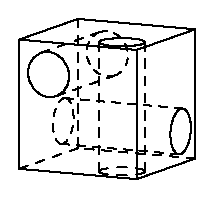
\includegraphics{asy/cube}
\end{wrapfigure}

More precisely, assume $(x,y,z)$ is the coordinate system on the cylindrical tunnel $\DD\z\times [0,1]$. 
Then the new metric is defined by
\[g=\phi\cdot [(dx)^2+ (dy)^2]+\tfrac1{\phi^2}\cdot (dz)^2,\]
where $\phi=\phi(x,y)$ is a positive smooth function on $\DD$ taking huge values around the center and equal to 1 near the boundary of $\DD$.


Gluing the opposite faces of the cube, we obtain a 3-dimensional torus with a smooth Riemannian metric.

Since the surface $S$ does not bound in $\TT^3=\mathbb{S}^1\times\mathbb{S}^1\times\mathbb{S}^1$,
one of the three coordinate projections $\TT^3\to\TT^2=\mathbb{S}^1\times\mathbb{S}^1$
induces a map of non-zero degree $S\to\TT^2$.
It follows that 
\[\area S\ge  \area(\DD,\phi\cdot [(dx)^2+ (dy)^2]).\]
For the right choice of the function $\phi$, the right hand side can be made larger than the given number $L$.
Hence the statement follows.
\qeds

I learned this problem from Dmirti Burago.
The following problem of Larry Guth \cite{guth} is closely related:

\begin{pr}
Given $\eps>0$, construct a bi-Lipschitz area-nonincreasing degree-one map 
\[[0,1]\times[0,1]\times [0,\eps]\to [0,\tfrac\eps7]\times [0,\tfrac\eps7]\times [0,\tfrac1{7\cdot\eps}].\]

\end{pr}


 
%%%%%%%%%%%%%%%%%%%%%%%%%%%%%%%%%%%%%%%%%%%%%%%%%%
\parbf{Normal exponential map.}
Assume there are $p\in M$ and $\eps>0$ 
such that the image of the normal exponential map to $L$
 does not intersect the ball $B(p,\eps)_M$; that is, no geodesic normal to $L$ crosses the ball.

Choose a positive real number $R$ such that $B(p,R)_M\cap L\ne \emptyset$.
The sectional curvature of $M$ in the ball $B(p,R)$
is bounded below by some constant, say $K$.

Given $q\in L$, denote by $v_q \in \T_qM$ the direction of a minimizing geodesic $[qp]$.
Note that $v_q\notin \mathrm{N}_qL$.
Moreover there is $\delta=\delta(\eps,K,R)\z>0$ 
such that for any point $q\in B(p,R)_M\cap L$,
and any normal vector $n\in \mathrm{N}_qL$,
we have 
\[\measuredangle (v_q,n)>\delta.\]
Otherwise the geodesic in the direction of $n$ would cross $B(p,\eps)_M$.

It follows that starting at any point $q\in B(p,R)_M\cap L$ 
one can construct a unit-speed curve $\gamma$ in $L$ such that 
\[|p-\gamma(t)|\le |p-q|-t\cdot\sin \delta.\]
Following $\gamma$ for some time brings us to $p$;
that is, $p\in L$, a contradiction.
\qeds

{

\begin{wrapfigure}{o}{28 mm}
\vskip-0 mm
\centering
\includegraphics{mppics/pic-404}
\end{wrapfigure}

The problem was suggested by Alexander Lytchak.

On the diagram you see an example of an immersion 
such that one point does not lie in the image of the corresponding normal exponential map.
It might be interesting to understand what type of subsets can be avoided by such images.

}
%%%%%%%%%%%%%%%%%%%%%%%%%%%%%%%%%%%%%%%%%%%%%%%%%%
\parbf{Symplectic squeezing in the torus.}
The embedding will be given as a composition of a linear symplectomorphism $\lambda$ 
with the quotient map $\phi\:\RR^4\to \TT^2\times\RR^2$ by the integral $(x_1,y_1)$-lattice.

\medskip

The composition $\phi\circ\lambda$ will preserve the symplectic structure;
it remains to find $\lambda$ such that the restriction $\phi\circ\lambda|_\Omega$
is injective.

Without loss of generality,
we can assume that $\Omega$ is a ball centered at the origin.
Choose an oriented 2-dimensional subspace $V$ of $\RR^4$ 
such that the integral of $\omega$ over 
$\Omega\cap V$ is a  positive number smaller than $\tfrac\pi4$. 

Note that there is a linear symplectomorphism $\lambda$ that maps planes parallel to $V$ to planes parallel to the $(x_1,y_1)$-plane, and that maps the disk $V\cap\Omega$ to a round disk.
It follows that the intersection of $\lambda(\Omega)$ 
with any plane parallel to the $(x_1,y_1)$-plane is a disk of radius at most $\tfrac 12$.
In particular $\phi\circ\lambda|_\Omega$
is injective.\qeds

This construction was given 
by Larry Guth \cite{guth-symplectic}
and attributed to Leonid Polterovich.

Note that according to Gromov's non-squeezing theorem \cite{gromov-pseudoholomorphic}, 
an analogous statement with $\CC\times \DD$ as the target space does not hold;
here $\DD\subset \CC$ is the open unit disk with the induced symplectic structure.
In particular, it shows that
the projection of $\lambda(\Omega)$ as above 
to the $(x_1,y_1)$-plane
cannot be made arbitrarily small.

%%%%%%%%%%%%%%%%%%%%%%%%%%%%%%%%%%%%%%%%%%%%%%%%%%
\parbf{Diffeomorphism test.}
Note that the map $f$ is an open immersion.

Let $h$ be the pullback metric on $M$ for $f\:M\to N$.
Clearly $h\ge g$.
In particular $(M,h)$ is complete and the map $f\:(M,h)\to N$ is a local isometry. 

Note that any local isometry between complete connected Riemannian manifolds of the same dimension is a covering map.
Since $N$ is simply connected, the result follows.
\qeds 

%???

%%%%%%%%%%%%%%%%%%%%%%%%%%%%%%%%%%%%%%%%%%%%%%%%%%
\parbf{Volume of tubular neighborhoods.}
This problem is a direct corollary of the so-called \emph{tube formula} given by Hermann Weyl \cite{weyl}.
It expresses the volume of the $r$-neighborhood of $M$ as a polynomial $p(r)$;
the coefficients of $p$, up to a multiplicative constant, are integrals over~$M$ of some quantities called the \emph{Lipschitz--Killing curvatures} --- these are certain scalars which can be expressed in terms of the curvature tensor at the given point.
The proof is done by straightforward calculations.

 

%%%%%%%%%%%%%%%%%%%%%%%%%%%%%%%%%%%%%%%%%%%%%%%%%%
%\begin{wrapfigure}[9]{r}{33 mm}
%\begin{lpic}[t(-0 mm),b(-0 mm),r(0 mm),l(0 mm)]{pics/tree(1)}
%\end{lpic}
%\end{wrapfigure}

\parbf{Disk.}
The following claim is the key step in the proof.
\begin{cl}{$({*})$}
Given a positive integer $n$, there is a binary tree $T_n$ embedded into the disk $\DD$ such that any null-homotopy of $\partial \DD$ passes a curve that intersects $n$ different edges.
\end{cl}


The proof of the claim can be done by induction on $n$; the base is trivial.
Assuming we constructed $T_{n-1}$, the tree $T_n$ can be obtained by identifying three endpoints of three copies of $T_{n-1}$.

\begin{figure}[h!]
\vskip0mm
\centering
\includegraphics{mppics/pic-406}
\end{figure}

Take $\eps=\tfrac1{10}$ and fix a large integer $n$.
Let us construct a metric on the disk $\DD$ with the embedded tree $T_n$ as in $({*})$ such that
its diameter and the length of its boundary are less than $1$
and  
the distance between any two edges of $T_n$ without a common vertex 
is at least $\eps$.

Choose a Riemannian metric $g$ on the cylinder $\mathbb S^1\times [0,1]$ such that
\begin{itemize}
\item The $\eps$-neighborhoods of the boundary components 
have product metrics.
\item Any vertical segment $x\times[0,1]$ has length $\tfrac 12$.
\item One of the boundary components has length $\eps$.
\item The other boundary component has length $2\cdot m\cdot \eps$, 
where $m$ is the number of edges in the tree $T_n$.
\end{itemize}
Equip $T_n$ with a length-metric so that each edge has length $\eps$.
Glue the cylinder $(\mathbb S^1\times [0,1],g)$ along its long boundary component to the tree $T_n$ by a piecewise isometry 
in such a way that the resulting space is homeomorphic to a disk and the obtained embedding of $T_n$ in $\DD$ is the same as in the claim $({*})$.

By $({*})$, any null-homotopy of the boundary passes a curve that intersects $n$ different edges of $T_n$.
By construction this curve is longer than $\tfrac{\eps}{10}\cdot n=\tfrac{1}{100}\cdot n$.

The obtained metric is not Riemannian, but is easy to smooth it while keeping this property.
Since $n$ is large the result follows.
\qeds
 
This example was constructed by Sidney Frankel and Mikhail Katz \cite{frankel-katz}.
 

%%%%%%%%%%%%%%%%%%%%%%%%%%%%%%%%%%%%%%%%%%%%%%%%%%
\parbf{Shortening homotopy.}
Set 
\[p=\gamma_0(0)\ \ \text{and}\ \  \ell_0=\length\gamma_0.\]

By a compactness argument,
there exists $\delta>0$ 
such that no geodesic loop based at $p$ has length in the interval $(L-D, L+D+\delta]$. 

Assume that $\ell_0\ge L+\delta$.
Choose $t_0\in [0,1]$ such that
\[\length\left(\gamma_0|_{[0,t_0]}\right)=L+\delta.\]
Let $\sigma$ be a minimizing geodesic from $\gamma(t_0)$
to $p$.
Note that $\gamma_0$ is homotopic to the concatenation 
\[\gamma_0'=\gamma_0|_{[0,t_0]}*\sigma*\bar\sigma*\gamma|_{[t_0,1]},\]
where $\bar\sigma$ denotes the backward parametrization of $\sigma$.

Applying a curve shortening process to the loop $\lambda_0=\gamma|_{[0,t_0]}*\sigma$, 
we get a  homotopy $\lambda_t$
relative to its endpoints 
from the loop $\lambda_0$ to a geodesic loop $\lambda_1$ at $p$.
From the above, 
\[\length\lambda_1\le L-D.\]

\begin{wrapfigure}{o}{31 mm}
\vskip-6mm
\centering
\includegraphics{mppics/pic-408}
\end{wrapfigure}

The concatenation $\gamma_t=\lambda_t*\bar\sigma*\gamma|_{[t_0,1]}$
is a homotopy
from $\gamma_0'$ to another curve $\gamma_1$.
From the construction it is clear that 
\begin{align*}
 \length \gamma_t&\le \length \gamma_0+2\cdot \length\sigma\le
 \\
 &\le \length \gamma_0+2\cdot D
\end{align*}
for any $t\in[0,1]$
and 
\begin{align*}
 \length \gamma_1&=\length\lambda_1+\length\sigma+\length\gamma|_{[t_0,1]}\le
\\ &\le L-D+D+\length\gamma-(L+\delta)=
\\ &=\ell_0 -\delta.
\end{align*}

Repeating the procedure sufficient number of times, we get curves $\gamma_2,\dots,\gamma_n$
connected by the needed homotopies so that 
$\ell_{i+1}\le\ell_i-\delta$ and $\ell_n\z< L+\delta$,
where $\ell_i=\length\gamma_i$.

If $\ell_n\le L$, we are done.
Otherwise repeat the argument again for $\delta'=\ell_n-L$.
\qeds

The problem is due to 
Alexander Nabutovsky 
and Regina Rotman \cite{nabutovsky-rotman}.


%%%%%%%%%%%%%%%%%%%%%%%%%%%%%%%%%%%%%%%%%%%%%%%%%%
\parbf{Convex hypersurface.}
First let us define the {}\emph{cone construction} of maps into $M$.

Let $\Delta'$ be a simplex 
with a vertex $v$.
Denote by $\Delta$ the facet in $\Delta'$ opposite to $v$.
Let $f\:\Delta\to M$ be a map such that $f(\Delta)\subset B(x,1)_M$ for some $x \in M$.
Given $w\in \Delta$, let $\gamma_w\:[0,1]\to M$ be the minimizing geodesic path from $x$ to  $f(w)$.
Since the injectivity radius of $M$ is at least $1$, the path $\gamma_w$ is uniquely defined.
The map $f'\:\Delta'\to M$ defined as 
\[f'\:(1-t)\cdot v+t\cdot w\mapsto \gamma_w(t)\] 
is called the {}\emph{cone over $f$} with vertex $x$. 

One may start with a map $f_0\:\Delta_0\to M$ and iterate the cone construction for the vertices $x_1,\dots x_k$,
to get a sequence of maps $f_i\:\Delta_i\to M$
as long as $f_{i-1}(\Delta_{i-1})\subset B(x_i,1)$.
Straightforward application of the triangle inequality 
shows that the latter conditions hold if 
$f_0(\Delta_0)\subset B(x_i,s)$ for each $i$ and $s<\tfrac2{2+k}$.

\medskip

Now we go back to the solution of the problem.

Choose a fine triangulation of $W$ so that $M$ becomes a sub-complex of $W$.
We can assume that the diameter of each simplex in $\tau$ is less than any given
$\eps>0$.
Furthermore, we can assume that all the vertices of $\tau$ can be colored with $m+2$ colors $(0,\dots, m+1)$
in such a way that the vertices of each simplex 
have different colors;
the latter can be achieved by passing to the barycentric subdivision of $\tau$.
Denote by $\tau_i$ the maximal $i$-dimensional sub-complex of $\tau$ 
with all the vertices colored by $0,\dots, i$.

Let $h$ be the maximal distance from points in $W$ to $M$.
For each vertex $v$ in $\tau$ 
choose a point $v'\in M$ at distance $\le h$.
Note that 
if $v$ and $w$ are vertices of one simplex,
then
\[|v'-w'|_M<2\cdot h+\eps.\]

Assume that $\tfrac{2}{m+3}>h$.
Choose positive $\eps<\tfrac{2}{m+3}-h$ and use it in the construction of the triangulation $\tau$ above.
Applying the iterated cone construction for each simplex of $\tau$
we get an extension of the map $v\mapsto v'$ defined on $\tau_0$ to $\tau_1,\dots\tau_{m+1}$.
According to the above estimates, the cone constructions are defined at each of the needed $m+1$ iterations.

This way we get 
to a retraction $W\to M$.
It follows that the fundamental class of $M$ vanishes in the homology ring of $M$, 
a contradiction. 
\qeds


This problem is a stripped version of the bound on filling radius given by Mikhael Gromov \cite{gromov-filling}.  

%%%%%%%%%%%%%%%%%%%%%%%%%%%%%%%%%%%%%%%%%%%%%%%%%%
\parbf{Almost constant function.}
Given a positive integer $m$,
denote by $\delta_m$ 
the expected value of $|x_1|$ for the random unit vector 
$\bm{x}\z=(x_1,\dots,x_m)\z\in\RR^m$ 
with respect to the uniform distribution.

Observe that $\delta_m\to 0$ as $m\to\infty$.
Indeed, from symmetry and Bunyakovsky inequality we get
\[
\tfrac1m=\tfrac1m\cdot\mathrm{E}(|\bm{x}|^2)
=\mathrm{E}(x_1^2)\ge \mathrm{E}(|x_1|)^2=\delta_m^2.
\]

Since $f$ is $1$-Lipschitz,
\[\mathrm{E}(|df(w)|)\le\delta_m\]
for a random vector $w$ in $\UU M$.


Note that 
\begin{align*}
|f\circ \gamma(1)-f\circ\gamma(0)|
&=
\left|\int\limits_0^1df(\gamma'(t))\cdot dt\right|\le \\
&\le \int\limits_0^1\left|df(\gamma'(t))\right|\cdot dt.
\end{align*}

Assume that $\gamma'(0)$
takes random value in $\UU M$.
By Liouville's theorem about phase volume, the same holds for $\gamma'(t)$
for any fixed $t$.
Therefore
\begin{align*}
\mathrm{E}(|f\circ \gamma(1)-f\circ\gamma(0)|)\le \mathrm{E}\left(\int\limits_0^1|df(\gamma'(t))|\cdot dt\right)\le\delta_m.
\end{align*}

By Markov's inequality,
the probability of the event 
\[|f\circ \gamma(1)-f\circ\gamma(0)|>\eps\]
is at most $\tfrac{\delta_m}{\eps}$.
Hence the result follows.
\qeds

I learned this problem from Mikhael Gromov.
It gives an example in the Riemannian world
of the so-called 
\index{concentration of measure}\emph{concentration of measure phenomenon}
\cite{milman-schechtman,ledoux}.
